
\chapter{Fractions}
\section{Fraction Definition and Equivalent Fractions}
\thispagestyle{fancy}

In this lesson, we will learn the definition of fractions, and how to change a fraction to an equivalent fraction.

\subsection{Definition of Fraction}

For a fraction like $\frac{2}{3}$, the number $2$ is the \textit{numerator}, and the number $3$ is the \textit{denominator}.

When we look at a fraction like $\frac{2}{3}$, we naturally look at the numerator ($2$) first. Actually, we should look at the denominator ($3$) first. Here is how to interpret $\frac{2}{3}$:

\begin{enumerate}
\item We cut the whole evenly into $3$ pieces.
\item We take $2$ of those pieces.
\end{enumerate}

\begin{center}
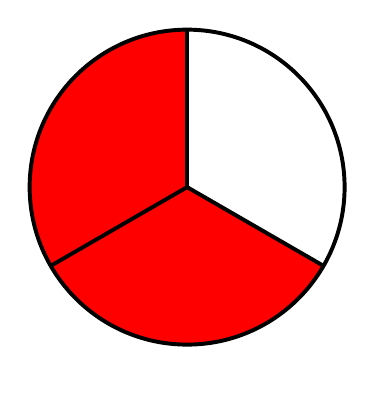
\begin{tikzpicture}
	\fill[red] (0,0) -- (0,2) arc (90:210:2cm) -- cycle;
	\fill[red] (0,0) -- (-2*0.8661,-2*0.5) arc (210:330:2cm) -- cycle;
	\draw[line width=0.5mm] (0,0) circle (2cm);
	\draw[line width=0.5mm] (0,0) -- (0,2);
	\draw[line width=0.5mm] (0,0) -- (2*0.8661,-2*0.5);
	\draw[line width=0.5mm] (0,0) -- (-2*0.8661,-2*0.5);
\end{tikzpicture}
\captionof{figure}{Red pieces in the pie represent $\frac{2}{3}$}
\end{center}

There are more ways to represent fractions graphically. For example:

\begin{center}
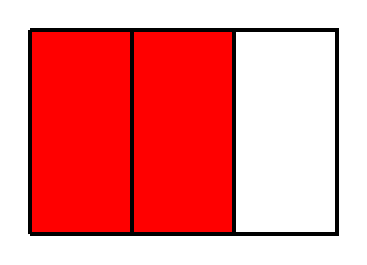
\begin{tikzpicture}
\draw[fill=red,line width=0.5mm] (0,0) -- (1.3*2,0) -- (1.3*2,1.3*2) -- (0,1.3*2);
\draw[line width=0.5mm] (1.3*1,0) -- (1.3*1,1.3*2);
\draw[line width=0.5mm] (0,0) -- (0,1.3*2);
\draw[line width=0.5mm] (1.3*2,0) -- (1.3*3,0) -- (1.3*3,1.3*2) -- (1.3*2,1.3*2);
\end{tikzpicture}
\captionof{figure}{Red pieces in the rectangle represent $\frac{2}{3}$}
\end{center}

Depending on the situations, we will use different shapes to represent fractions.

\subsection{Equivalent Fractions}
Let's look at the following two graphs:

\begin{center}
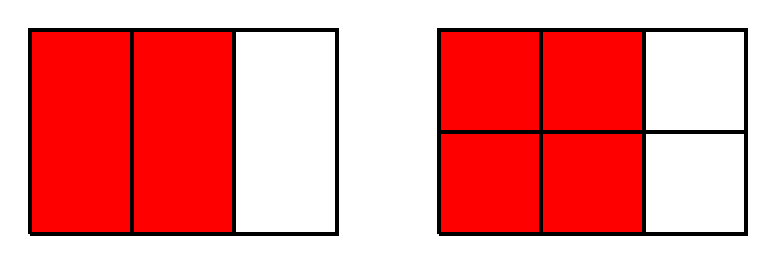
\begin{tikzpicture}

\draw[fill=red,line width=0.5mm] (0,0) -- (1.3*2,0) -- (1.3*2,1.3*2) -- (0,1.3*2) -- (0,0);
\draw[line width=0.5mm] (1.3*1,0) -- (1.3*1,1.3*2);
\draw[line width=0.5mm] (1.3*2,0) -- (1.3*3,0) -- (1.3*3,1.3*2) -- (1.3*2,1.3*2);

\draw[fill=red,line width=0.5mm] (1.3*4,0) -- (1.3*6,0) -- (1.3*6,1.3*2) -- (1.3*4,1.3*2) -- (1.3*4,0);
\draw[line width=0.5mm] (1.3*5,0) -- (1.3*5,1.3*2);
\draw[line width=0.5mm] (1.3*4,1.3*1) -- (1.3*7,1.3*1);
\draw[line width=0.5mm] (1.3*6,0) -- (1.3*7,0) -- (1.3*7,1.3*2) -- (1.3*6,1.3*2);

\end{tikzpicture}
\captionof{figure}{Compare $\frac{2}{3}$ and $\frac{4}{6}$}
\end{center}

The graph on the left side represents $\frac{2}{3}$, and the graph on the right side represents $\frac{4}{6}$. We can see they actually cover the same area. In other words:
\[ \frac{2}{3}=\frac{4}{6} \]

The difference is that the rectangle on the right side is cut into twice as many pieces as the rectangle on the left side. Let's look at this equation:
\[ \frac{2}{3}=\frac{2\cdot2}{3\cdot2}=\frac{4}{6} \]

To change $\frac{2}{3}$ to $\frac{4}{6}$, we multiply $2$ in both the numerator and denominator. This implies we cut the rectangle into twice as many pieces ($6$), and take twice as many pieces ($4$). The value of the fraction didn't change!

For $\frac{2}{3}$, if we cut the rectangle into $3$ times as many pieces, and take $3$ times as many pieces, the fraction's value would not change, either:
\[ \frac{2}{3}=\frac{2\cdot3}{3\cdot3}=\frac{6}{9} \]

Let's look at a graphic representation of this equation:

\begin{center}
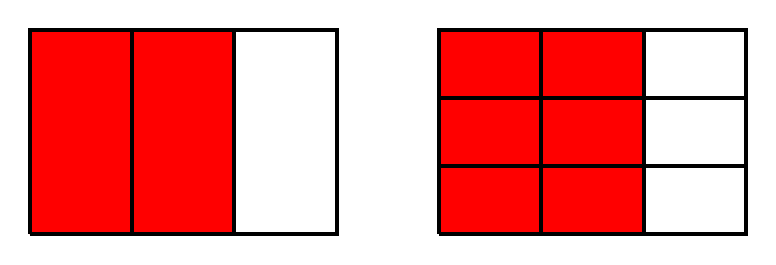
\begin{tikzpicture}

\draw[fill=red,line width=0.5mm] (0,0) -- (1.3*2,0) -- (1.3*2,1.3*2) -- (0,1.3*2) -- (0,0);
\draw[line width=0.5mm] (1.3*1,0) -- (1.3*1,1.3*2);
\draw[line width=0.5mm] (1.3*2,0) -- (1.3*3,0) -- (1.3*3,1.3*2) -- (1.3*2,1.3*2);

\draw[fill=red,line width=0.5mm] (1.3*4,0) -- (1.3*6,0) -- (1.3*6,1.3*2) -- (1.3*4,1.3*2) -- (1.3*4,0);
\draw[line width=0.5mm] (1.3*5,0) -- (1.3*5,1.3*2);
\draw[line width=0.5mm] (1.3*4,1.3*2/3) -- (1.3*7,1.3*2/3);
\draw[line width=0.5mm] (1.3*4,1.3*4/3) -- (1.3*7,1.3*4/3);
\draw[line width=0.5mm] (1.3*6,0) -- (1.3*7,0) -- (1.3*7,1.3*2) -- (1.3*6,1.3*2);

\end{tikzpicture}
\captionof{figure}{$\frac{2}{3}$ = $\frac{6}{9}$}
\end{center}

Here is the rule: If we multiply the same number in both the numerator and denominator of a fraction, the fraction's value doesn't change. For example, $\frac{2}{3}=\frac{2\cdot2}{3\cdot2}=\frac{4}{6}$, and $\frac{2}{3}=\frac{2\cdot3}{3\cdot3}=\frac{6}{9}$.

\begin{myexample}
Write a few equivalent fractions of $\frac{4}{5}$.
\end{myexample}
\begin{solution}
\[
\begin{aligned}[t]
   &\frac{4}{5}=\frac{4\cdot2}{5\cdot2}=\frac{8}{10} \\
   &\frac{4}{5}=\frac{4\cdot3}{5\cdot3}=\frac{12}{15} \\
   &\frac{4}{5}=\frac{4\cdot4}{5\cdot4}=\frac{16}{20} \\
   &\frac{4}{5}=\frac{4\cdot5}{5\cdot5}=\frac{20}{25} \\
   &...
\end{aligned}
\]
\end{solution}

\begin{myexample}
Change $\frac{2}{3}$ to an equivalent fraction with the denominator of $12$.
\end{myexample}
\begin{solution}
The question asks:
\[ \frac{2}{3}=\frac{?}{12} \]
To change the denominator from $3$ to $12$, we need to do $3\cdot4=12$. If we multiply the denominator with $4$, we must do the same to the numerator. We have:
\[ \frac{2}{3}=\frac{2\cdot4}{3\cdot4}=\frac{8}{12} \]
\end{solution}

Similarly, we can reduce fractions by dividing the same number in both the numerator and denominator:
\[
\begin{aligned}[t]
   &\frac{4}{6}=\frac{4\div2}{6\div2}=\frac{2}{3} \\
   &\frac{6}{9}=\frac{6\div3}{9\div3}=\frac{2}{3} \\
   &\frac{20}{25}=\frac{20\div5}{25\div5}=\frac{4}{5} \\
   &...
\end{aligned}
\]

How do we know which number to divide when we reduce fractions? Think about prime numbers: $2,3,5,7,11...$. Try prime numbers one by one.

\begin{myexample}
Reduce the fraction $\frac{30}{36}$.
\end{myexample}
\begin{solution}
\[
\begin{aligned}[t]
   &\phantom{{}=} \frac{24}{36} \\
   &= \frac{24\div2}{36\div2} &\phantom{=====}\text{2 goes into both 24 and 36.} \\
   &= \frac{12}{18} \\
   &= \frac{12\div2}{18\div2} &\phantom{=====}\text{2 goes into both 12 and 18.} \\
   &= \frac{6}{9} \\
   &= \frac{6\div3}{9\div3} &\phantom{=====}\text{3 goes into both 6 and 9.} \\
   &= \frac{2}{3} &\text{No more prime numbers go into both 2 and 3.}\\
\end{aligned}
\]
\end{solution}

You only need to memorize the first $5$ prime numbers: $2,3,5,7,11$. Rarely would an instructor expect you to see the prime number $13$ goes into two numbers. Actually, to see whether $7$ goes into a number, usually we resort to a calculator.

If we can reduce a fraction, we must do so! We don't allow reducible fractions like $\frac{2}{4}$ and $\frac{3}{9}$ as the final answer of a problem. 

There is an easier way to reduce $\frac{24}{36}$:
\[ \frac{24}{36}=\frac{24\div12}{36\div12}=\frac{2}{3} \]
If you can see $12$ goes into both $24$ and $36$, you can reduce $\frac{24}{36}$ in one step. However, if you cannot see it, simply go through the list of prime numbers one by one, $2,3,5,7,11...$, you can still reduce $\frac{24}{36}$ to $\frac{2}{3}$.

\begin{myexample}
Reduce the fraction $\frac{42}{126}$.
\end{myexample}
\begin{solution}
\[
\begin{aligned}[t]
   &\phantom{{}=} \frac{42}{126} \\
   &= \frac{42\div2}{126\div2} &\phantom{=====}\text{2 goes into both 42 and 126.} \\
   &= \frac{21}{63} \\
   &= \frac{21\div3}{63\div3} &\phantom{=====}\text{3 goes into both 21 and 63.} \\
   &= \frac{7}{21} \\
   &= \frac{7\div7}{21\div7} &\phantom{=====}\text{7 goes into both 7 and 21.} \\
   &= \frac{1}{3}\\
\end{aligned}
\]
\end{solution}

Here are a few special cases in fraction reduction. Remember: The fraction line has the same function as the division symbol.

\[
\begin{aligned}[t]
   &\frac{10}{10}=10\div10=1 \\
   &\frac{10}{1}=10\div1=10 \\
   &\frac{10}{0}=10\div0=\text{undefined} \\
   &\frac{0}{10}=0\div10=0 \\
\end{aligned}
\]

We can easily change a fraction to a decimal with a simple division: $\frac{1}{2}=1\div2=0.5$. We will cover this in the decimal chapter.

\subsection{Compare Fractions}
It's easy to understand that $\frac{2}{3}>\frac{1}{3}$, and $\frac{3}{10}<\frac{7}{10}$. How would we compare fractions when the denominators are different? Like $\frac{5}{6}$ and $\frac{7}{8}$?

Now that we learned how to change a fraction to its equivalent, we can change the denominators to the same number and then compare them.

\begin{myexample}
Compare $\frac{5}{6}$ and $\frac{7}{8}$.
\label{ex:u3l1CompareFractions}
\end{myexample}
\begin{solution}
Since $6\cdot8=48$, we know both $6$ and $8$ go into $48$, so we will change both denominators to $48$:
\[ \frac{5}{6} = \frac{5\cdot8}{6\cdot8} = \frac{30}{48} \text{ and } \frac{7}{8} = \frac{7\cdot6}{8\cdot6} = \frac{42}{48} \]

\textbf{Conclusion:} Now we can tell $\frac{5}{6}<\frac{7}{8}$.

If you can see both $6$ and $8$ go into $24$, you can avoid dealing with bigger numbers, but the result would be the same. In that case, you would do:
\[ \frac{5}{6} = \frac{5\cdot4}{6\cdot4} = \frac{20}{24} \text{ and } \frac{7}{8} = \frac{7\cdot3}{8\cdot3} = \frac{21}{24} \]

The conclusion stays the same: $\frac{7}{8}$ is bigger.
\end{solution}

\subsection{Fractions on Number Line}
The following figures show how to locate fractions on the number line. These figures are pretty self-explanatory. We need to count each unit (from 0 to 1) is cut into how many segments.

\begin{center}
\begin{tikzpicture}
% a straight line segment
\draw [<->] (0,0) -- (12,0);
% the ticks and their labels
\foreach \x  in {1,...,11}
  \draw[xshift=\x cm] (0pt,2pt) -- (0pt,-1pt);
\node[fill=black,draw=black,circle,inner sep=2pt,label=below:{$0$}] at (6,0) {};
\node[fill=black,draw=black,circle,inner sep=2pt,label=below:{$1$}] at (11,0) {};
\node[fill=black,draw=black,circle,inner sep=2pt,label=below:{$-1$}] at (1,0) {};
\node[fill=red,draw=red,circle,inner sep=2pt,label=above:{$\frac{1}{5}$}] at (7,0) {};
\end{tikzpicture}

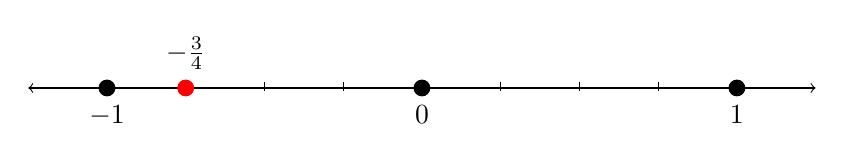
\begin{tikzpicture}
% a straight line segment
\draw [<->] (0,0) -- (10,0);
% the ticks and their labels
\foreach \x  in {1,...,9}
  \draw[xshift=\x cm] (0pt,2pt) -- (0pt,-1pt);
\node[fill=black,draw=black,circle,inner sep=2pt,label=below:{$0$}] at (5,0) {};
\node[fill=black,draw=black,circle,inner sep=2pt,label=below:{$1$}] at (9,0) {};
\node[fill=black,draw=black,circle,inner sep=2pt,label=below:{$-1$}] at (1,0) {};
\node[fill=red,draw=red,circle,inner sep=2pt,label=above:{$-\frac{3}{4}$}] at (2,0) {};
\end{tikzpicture}

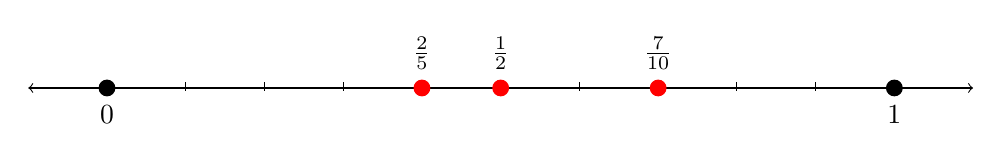
\begin{tikzpicture}
% a straight line segment
\draw [<->] (0,0) -- (12,0);
% the ticks and their labels
\foreach \x  in {1,...,11}
  \draw[xshift=\x cm] (0pt,2pt) -- (0pt,-1pt);
\node[fill=black,draw=black,circle,inner sep=2pt,label=below:{$0$}] at (1,0) {};
\node[fill=black,draw=black,circle,inner sep=2pt,label=below:{$1$}] at (11,0) {};
\node[fill=red,draw=red,circle,inner sep=2pt,label=above:{$\frac{7}{10}$}] at (8,0) {};
\node[fill=red,draw=red,circle,inner sep=2pt,label=above:{$\frac{1}{2}$}] at (6,0) {};
\node[fill=red,draw=red,circle,inner sep=2pt,label=above:{$\frac{2}{5}$}] at (5,0) {};
\end{tikzpicture}
\captionof{figure}{Locate fractions on number line}

\end{center}

On the last number line, note that the segment from $0$ to $1$ is cut evenly into $10$ pieces, implying each piece represents $\frac{1}{10}$. The first red dot is $4$ pieces away from $0$, which represents $\frac{4}{10}$. We must reduce the fraction: $\frac{4}{10}=\frac{2}{5}$.

Similarly, the second red dot represents $\frac{5}{10}$. We must again reduce the fraction: $\frac{5}{10}=\frac{1}{2}$.

The third red dot represents $\frac{7}{10}$. We cannot reduce this fraction.

\subsection{Summary}
Let's review what we learned in this lesson:
\begin{itemize}
\item To understand a fraction like $\frac{2}{3}$, we look at the denominator $3$ first, and then look at the numerator $2$. For $\frac{2}{3}$, we cut the whole evenly into $3$ pieces, and then take $2$ of those pieces.
\item If we multiply the same number in both the numerator and denominator of a fraction, the fraction's value doesn't change. For example, 
\[ \frac{2}{3}=\frac{2\cdot2}{3\cdot2}=\frac{4}{6} \]
\item If we divide the same number in both the numerator and denominator of a fraction, the fraction's value doesn't change. For example, 
\[ \frac{4}{6}=\frac{4\div2}{6\div2}=\frac{2}{3} \]
\item When we compare two fractions with different denominators, we can change the denominators to the same number, and then compare the numerators, like in \cref{ex:u3l1CompareFractions}.
\end{itemize}